\documentclass[11pt]{article}

\usepackage[letterpaper,margin=0.82in,headheight=15pt]{geometry}
\usepackage[T1]{fontenc}
\usepackage[utf8]{inputenc}
\usepackage{lmodern}
\usepackage{microtype}
\usepackage{graphicx}
\usepackage{booktabs}
\usepackage{tabularx}
\usepackage{array}
\usepackage{siunitx}
\usepackage{xcolor}
\usepackage{hyperref}
\usepackage{fancyhdr}
\usepackage{titlesec}
\usepackage{caption}
\usepackage{enumitem}
\usepackage{float}

\definecolor{navy}{HTML}{17365D}
\definecolor{blue}{HTML}{2E75B6}
\definecolor{lightblue}{HTML}{D9EAF7}
\definecolor{orange}{HTML}{D55E00}
\definecolor{graytext}{HTML}{555555}

\hypersetup{
  colorlinks=true,
  linkcolor=navy,
  urlcolor=blue,
  pdftitle={Building Vibration Measurement Analysis},
  pdfsubject={Laboratory vibration ranking and optical-table assessment}
}
\graphicspath{{../figures/}}
\sisetup{
  scientific-notation=true,
  round-mode=figures,
  round-precision=3,
  exponent-product=\times,
  detect-all
}
\DeclareSIUnit{\sqrthertz}{\hertz\tothe{0.5}}

\pagestyle{fancy}
\fancyhf{}
\lhead{\textcolor{graytext}{Building Vibration Assessment}}
\rhead{\textcolor{graytext}{Physics Laboratories}}
\cfoot{\thepage}
\renewcommand{\headrulewidth}{0.4pt}

\titleformat{\section}{\Large\bfseries\color{navy}}{\thesection}{0.7em}{}
\titleformat{\subsection}{\large\bfseries\color{blue}}{\thesubsection}{0.7em}{}
\captionsetup{font=small,labelfont=bf}
\setlist{nosep,leftmargin=1.5em}
\setlength{\parindent}{0pt}
\setlength{\parskip}{0.55em}
\renewcommand{\arraystretch}{1.15}

\newcommand{\asdunit}{\si{\meter\per\second\squared\per\sqrthertz}}
\newcommand{\confidence}[1]{\textcolor{navy}{\textbf{#1}}}

\begin{document}

\hypersetup{pageanchor=false}
\begin{titlepage}
  \centering
  \vspace*{1.2in}
  {\color{navy}\rule{\textwidth}{1.2pt}\par}
  \vspace{0.45in}
  {\Huge\bfseries Building Vibration Measurement Analysis\par}
  \vspace{0.18in}
  {\Large Laboratory ranking and optical-table performance\par}
  \vspace{0.45in}
  {\color{navy}\rule{\textwidth}{1.2pt}\par}
  \vfill
  \begin{tabular}{rl}
    \textbf{Source workbook:} & \texttt{FinalReportData.xlsx}\\
    \textbf{Measurements:} & 15 spectra in 5 measured rooms\\
    \textbf{Spectral range:} & 0--250.25 Hz at 0.48877 Hz resolution\\
    \textbf{Report date:} & July 24, 2026\\
  \end{tabular}
  \vfill
  {\large Prepared for vibration-sensitive experimental work\par}
\end{titlepage}

\hypersetup{pageanchor=true}
\pagenumbering{roman}
\tableofcontents
\clearpage
\pagenumbering{arabic}

\section{Summary}

\textbf{Recommendation.} PHYS 244 has the lowest measured representative-floor
RMS acceleration. Over 0.5--250 Hz, it is
\SI{4.52e-3}{\meter\per\second\squared}. PHYS 245 is second at
\SI{5.35e-3}{\meter\per\second\squared} (+18.3\%, +1.46 dB), and the main
Titan laboratory is third at
\SI{6.02e-3}{\meter\per\second\squared} (+33.2\%, +2.49 dB).

Titan has the lowest median ASD,
\SI{2.26e-4}{\meter\per\second\squared\per\sqrthertz}, and is especially
quiet between narrow spectral lines. Its larger total RMS is driven mainly
by the heating-plant-coupled 29.8 Hz line. PHYS 244 is therefore the safer
general recommendation, while Titan remains attractive for experiments with
little mechanical response near 29.8 Hz.

Herzog is the least favorable floor location. Its RMS is
\SI{2.23e-2}{\meter\per\second\squared}, 4.92 times PHYS 244
(+13.85 dB), and its 29.8 Hz line reaches
\SI{2.29e-2}{\meter\per\second\squared\per\sqrthertz}. PHYS 111 is also
elevated and ranks fourth.

Optical-table performance is frequency dependent. The Herzog table reduces
total RMS by 72.9\% (-11.35 dB) from its unusually noisy floor, reaching
\SI{6.03e-3}{\meter\per\second\squared}. The PHYS 245 floated table has
21.0\% higher total RMS than the PHYS 245 floor (+1.66 dB), driven partly by
a 17.6 Hz feature.

\section{Analysis methodology}

The numerical spectrum columns are acceleration amplitude spectral density
(ASD), in \asdunit. For a frequency band containing bins of width
$\Delta f$, the band-limited RMS acceleration is
\[
  a_{\mathrm{RMS}} =
  \sqrt{\sum_k \mathrm{ASD}(f_k)^2\,\Delta f}.
\]

The principal room comparison integrates the complete measured spectrum from
0.5 to 250 Hz. Band results are calculated for 0.5--5, 5--10, 10--20,
20--50, 50--100, and 100--250 Hz. Individual lines are retained in the
calculation as measured vibration.

The measurements are single spectra rather than independent repeated trials.
Small differences should therefore be treated as descriptive, while the large
separation between Herzog or PHYS 111 and the quieter rooms is robust.

\section{Results by laboratory}

\begin{figure}[H]
\centering
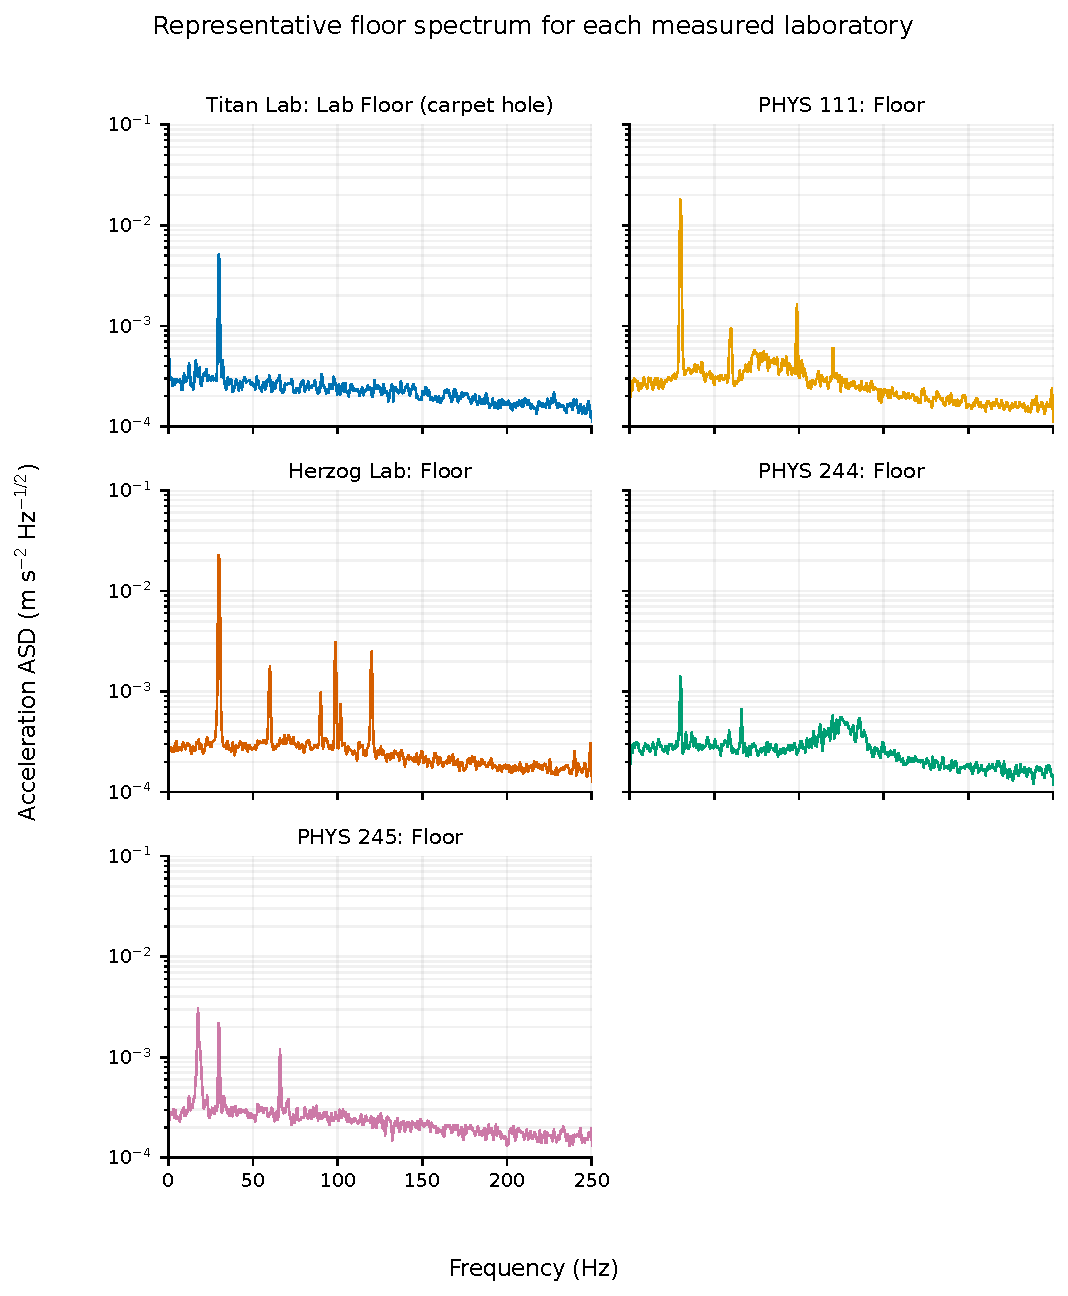
\includegraphics[width=0.93\linewidth]{representative_spectra_by_room.pdf}
\caption{Representative floor spectrum for each measured laboratory. All
panels use common logarithmic amplitude limits, and no smoothing is applied.}
\label{fig:representative}
\end{figure}

\subsection{Titan laboratory}

The main Titan floor has the lowest median ASD of the five representative
floors. Its integrated RMS is
\SI{6.02e-3}{\meter\per\second\squared}; the heating-plant-coupled 29.8 Hz
line is the principal reason it does not rank first by total RMS. Titan remains
the cleanest broadband environment between the narrow lines.

\subsection{PHYS 111}

The PHYS 111 floor ranks fourth at
\SI{1.75e-2}{\meter\per\second\squared}. The counter along the Herzog wall is
higher at approximately \SI{2.24e-2}{\meter\per\second\squared}, consistent
with stronger local structural motion near that boundary.

The optical table near the wall reduces total RMS to
\SI{1.02e-2}{\meter\per\second\squared}. The table-door run is anomalously
high and is not used to characterize normal table performance.

\subsection{Herzog laboratory}

Herzog has the highest representative-floor RMS,
\SI{2.23e-2}{\meter\per\second\squared}, and the largest representative-floor
29.8 Hz amplitude. Its back counter is higher still in total RMS. These
measurements agree with the observation that vibration is readily perceptible
in this room.

The optical-table run is substantially quieter at
\SI{6.03e-3}{\meter\per\second\squared}, close to the Titan floor value.
The table's float status was not recorded.

\subsection{PHYS 244}

PHYS 244 has the lowest representative-floor RMS,
\SI{4.52e-3}{\meter\per\second\squared}. Its wooden table is 17.4\% higher
than the floor and contains a stronger 66.0 Hz feature. The floor is therefore
the preferred measured surface in this room.

\subsection{PHYS 245}

The PHYS 245 floor ranks second at
\SI{5.35e-3}{\meter\per\second\squared}. The unfloated optical table is
\SI{5.92e-3}{\meter\per\second\squared}; the floated AFM table is
\SI{6.48e-3}{\meter\per\second\squared}. The 17.6 Hz amplification on the
floated table is large enough to merit attention when judging its performance.

\section{Optical-table isolation performance}

\begin{figure}[H]
\centering
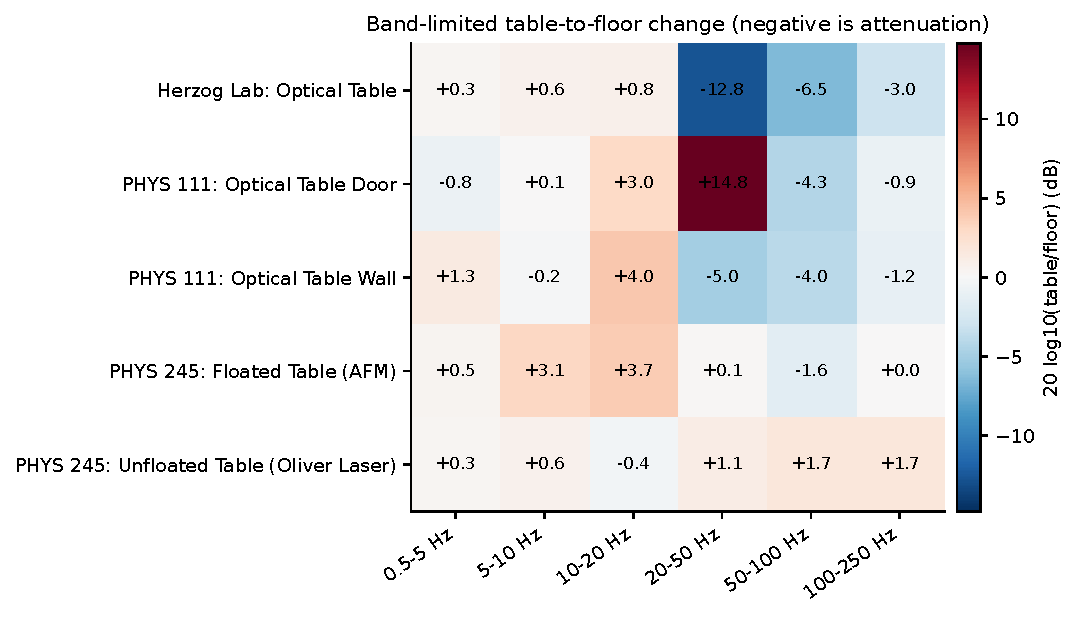
\includegraphics[width=0.95\linewidth]{optical_table_attenuation_heatmap.pdf}
\caption{Band-limited table-to-floor change. Negative dB values are
attenuation; positive values are amplification.}
\label{fig:attenuation}
\end{figure}

\begin{table}[H]
\centering
\caption{Integrated 0.5--250 Hz table-to-floor comparisons.}
\scriptsize
\begin{tabular}{rllllll}
\toprule
Room & Table location & Floor RMS & Table RMS & Ratio & Reduction (\%) & Change (dB) \\
\midrule
PHYS 111 & Optical Table Wall & 0.0175 & 0.0102 & 0.58 & +41.7 & -4.7 \\
PHYS 111 & Optical Table Door & 0.0175 & 0.0926 & 5.30 & -430.4 & +14.5 \\
Herzog Lab & Optical Table & 0.0223 & 0.00603 & 0.27 & +72.9 & -11.3 \\
PHYS 245 & Floated Table (AFM) & 0.00535 & 0.00648 & 1.21 & -21.0 & +1.7 \\
PHYS 245 & Unfloated Table (Oliver Laser) & 0.00535 & 0.00592 & 1.11 & -10.6 & +0.9 \\
\bottomrule
\end{tabular}

\label{tab:table-summary}
\end{table}

The Herzog table gives the largest overall reduction because the Herzog floor
starts from the largest vibration level. Its table spectrum is nevertheless
not the quietest surface measured: its total RMS remains close to Titan and
above the PHYS 244 and PHYS 245 floor measurements.

The PHYS 111 table-wall run provides -4.69 dB overall. The PHYS 245 floated
table suppresses the 66.0 Hz floor feature but amplifies the 17.6 Hz feature,
so its total RMS is +1.66 dB relative to the floor.

\begin{figure}[H]
\centering
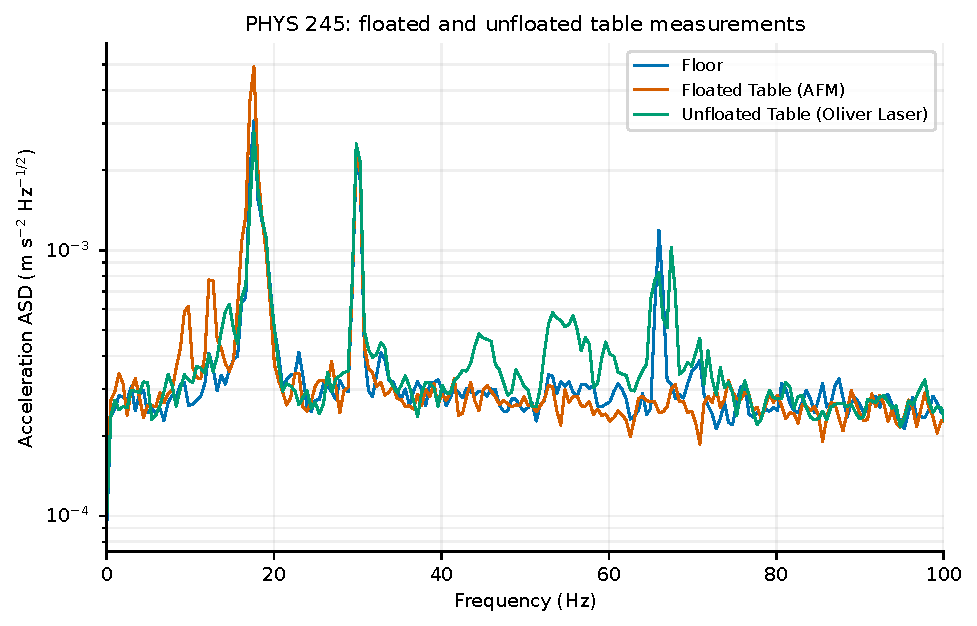
\includegraphics[width=0.88\linewidth]{phys245_floated_unfloated_floor.pdf}
\caption{PHYS 245 floor, floated AFM table, and unfloated optical table. The
floated table suppresses the 66 Hz feature but amplifies the 17.6 Hz feature.}
\label{fig:phys245}
\end{figure}

\section{Herzog freezer check}

\begin{figure}[H]
\centering
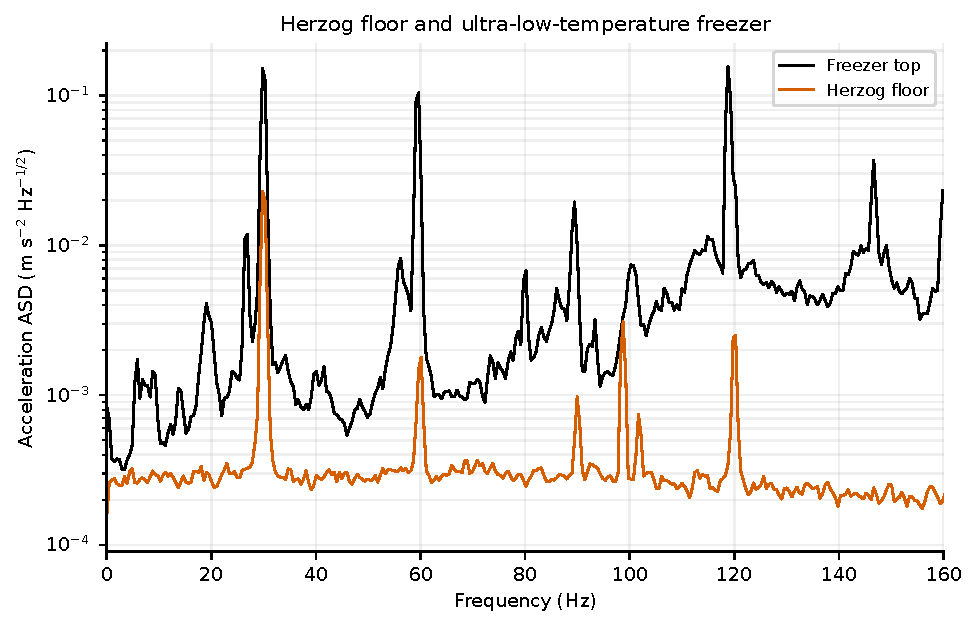
\includegraphics[width=0.9\linewidth]{herzog_phys111_freezer_comparison.pdf}
\caption{Herzog floor and the spectrum measured directly on top of the
ultra-low-temperature freezer.}
\label{fig:freezer}
\end{figure}

The freezer-top spectrum is much larger and contains many strong local lines,
but those features do not appear at comparable strength on the Herzog floor.
The measured freezer noise is therefore not coupling significantly into the
floor spectrum.

\section{Laboratory ranking}

\begin{table}[H]
\centering
\caption{Representative-floor ranking. Median ASD is in \asdunit.}
\scriptsize
\begin{tabular}{rllll}
\toprule
Rank & Room & Floor location & RMS (m/s$^2$) & Median ASD \\
\midrule
1 & PHYS 244 & Floor & 0.00452 & 0.000258 \\
2 & PHYS 245 & Floor & 0.00535 & 0.000228 \\
3 & Titan Lab & Lab Floor (carpet hole) & 0.00602 & 0.000226 \\
4 & PHYS 111 & Floor & 0.0175 & 0.000253 \\
5 & Herzog Lab & Floor & 0.0223 & 0.000241 \\
\bottomrule
\end{tabular}

\label{tab:ranking}
\end{table}

PHYS 244 ranks first under the complete integrated metric. PHYS 245 and Titan
are close enough that experiment-specific mechanical response could reverse
their preferred order. Herzog and PHYS 111 are clearly separated from the
three quieter rooms.

\section{Recommendations}

\begin{enumerate}
  \item \textbf{Use PHYS 244 for a general-purpose vibration-sensitive
  installation} based on the lowest measured floor RMS.
  \item \textbf{Keep Titan as a strong alternate} when its lower broadband
  background is more important than its 29.8 Hz line.
  \item \textbf{Use optical isolation in Herzog only with verification.}
  The table reduces the unusually large floor motion, but its absolute table
  level is not lower than the quietest room floors.
  \item \textbf{Inspect the PHYS 245 floated AFM table} if the experiment is
  sensitive near 17.6 Hz.
  \item \textbf{Avoid the Herzog and PHYS 111 floors for the most sensitive
  experiments} unless additional, verified isolation is used.
\end{enumerate}

\section{Conclusions}

\begin{itemize}
  \item PHYS 244 has the lowest representative-floor integrated RMS.
  \item Titan has the lowest median floor ASD but a strong
  heating-plant-coupled 29.8 Hz line.
  \item Herzog is the highest-vibration representative floor, and PHYS 111 is
  also elevated.
  \item The Herzog table strongly reduces its floor motion, while the PHYS 245
  floated table amplifies the 17.6 Hz region in the supplied run.
  \item The freezer's strong local vibration is not coupling significantly
  into the Herzog floor spectrum.
\end{itemize}

\end{document}
